A flow in a cavity where the side and bottom walls are fixes and 
the cover moves at a constant velocity such as \textit{$U_{top}=1$} 
is known as \textit {Lid-driven Cavity flow}.
In addition to 
yhe streamfunction is set null value in all boundary, 
because there is no volumetric flux crossing the boundaries 
in lid-driven cavity flow.
The \ref{cavity} presents schematically this flow and 
the expected velocity field.

\vspace{1cm}
\begin{figure}[H]
\begin{center}
\begin{tikzpicture}[scale=1.1]
 \draw [pattern=north east lines] (0,-0.1) -- (3,-0.1) -- (3,3) -- (2.9,3) -- (2.9,0) -- (0.1,0) -- (0.1,3) -- (0,3) -- cycle;
 \draw [pattern=north east lines] (-0.1,3) -- (-0.1,3.1) -- (3.1,3.1) -- (3.1,3) -- cycle;

 \draw [->,thick] (3.2,3.05)--(4.2,3.05) node[above] {$U_{top}$};

 \draw [->,thick] (2.4,2.4) arc (45:-180:1.2);
 
 \draw [->,thick] (-2,-0.1)--(-2,1.5) node[left] {$y$};
 \draw [->,thick] (-2.1,0)--(-0.5,0) node[below] {$x$};

\end{tikzpicture}
\end{center}
\caption{Lid-driven Cavity Flow}
\label{cavity}
\end{figure}

\bigskip
The benchmark problem were simulated with the following 
Reynolds numbers (\textit{Re}): 10, 100, 400 and 1000.
The \ref{velocity vx cavity} and \ref{velocity vy cavity} 
prsent the profile of $u$ and $v$, respectively,
for steady state in several Reynolds number. 
They were compared with 
Ghia et al. (1982) \cite{ghia1982} and 
Marchi et al. (2009) \cite{marchi2009}. 
The domain was discretized using a linear triangular mesh 
with 1563 nodes and 2988 elements.

\begin{center}
\begin{figure}[H]
     \centering
     \begin{minipage}{.5\linewidth}
      \centering
      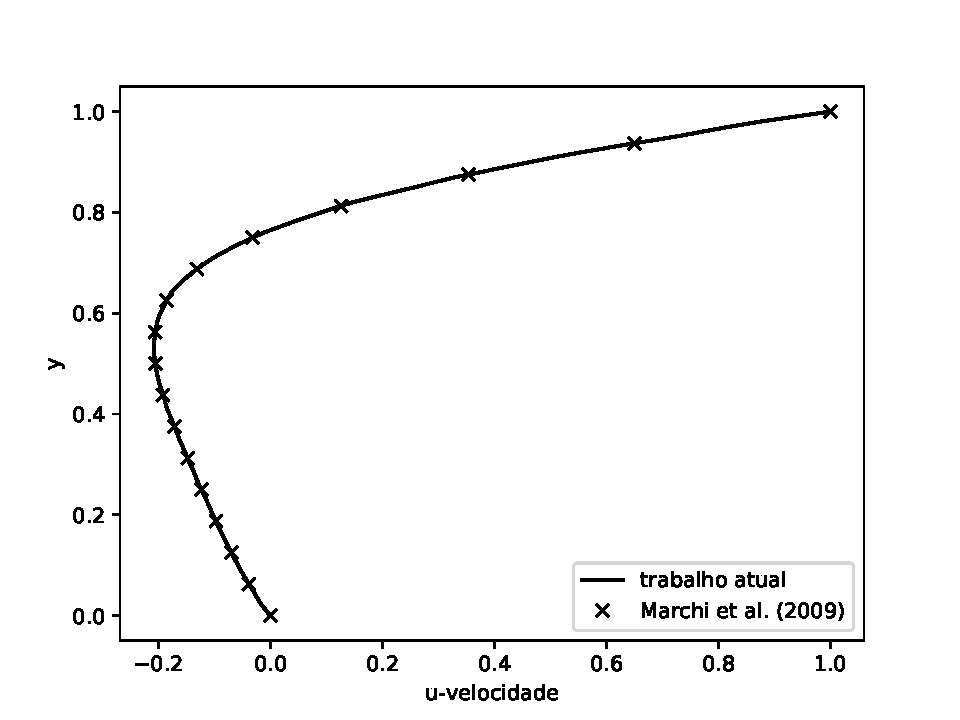
\includegraphics[scale=0.53]{./02_chaps/cap_validation/figure/Re_10_u_profile.pdf}\\
      (a)
     \end{minipage}%
     \begin{minipage}{.5\linewidth}
      \centering
      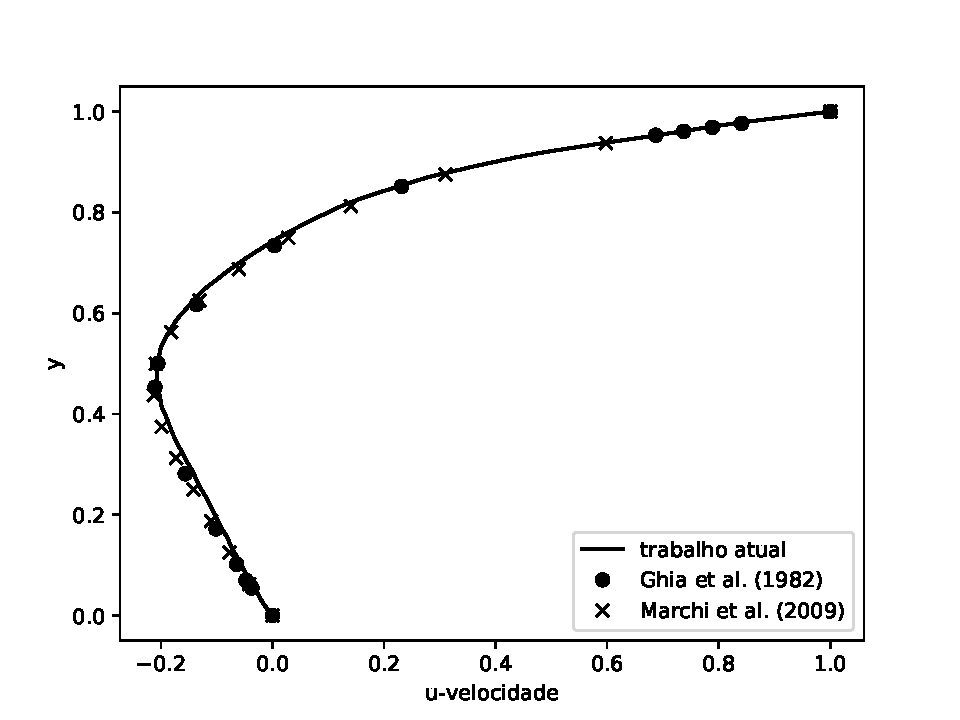
\includegraphics[scale=0.53]{./02_chaps/cap_validation/figure/Re_100_u_profile.pdf}\\
      (b)
     \end{minipage}
     \begin{minipage}{.5\linewidth}
      \centering
      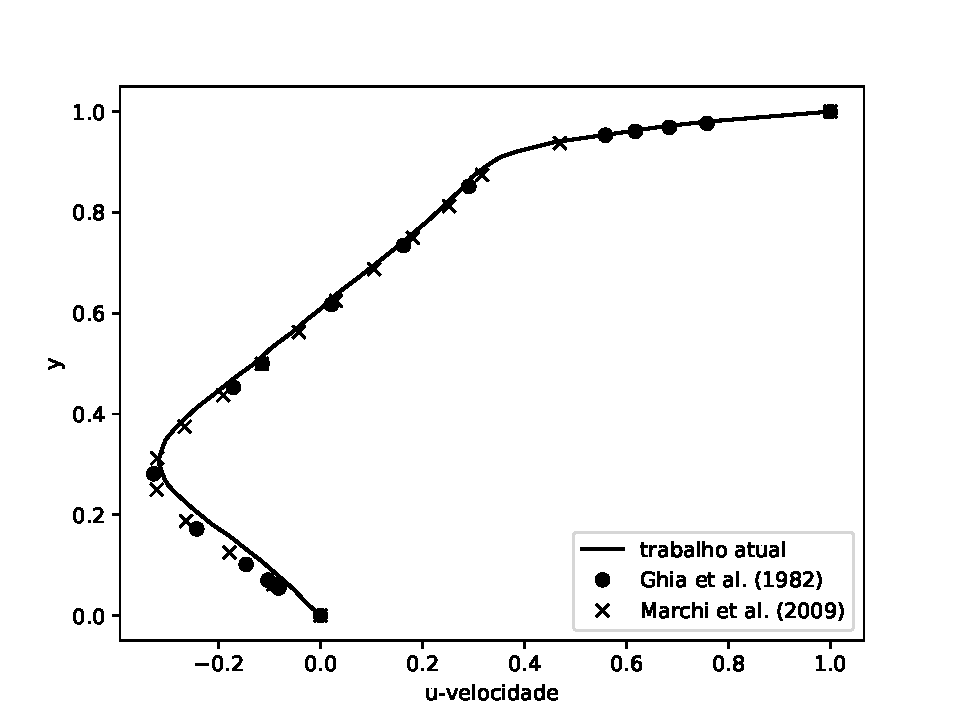
\includegraphics[scale=0.53]{./02_chaps/cap_validation/figure/Re_400_u_profile.pdf}\\
      (c)
     \end{minipage}%
     \begin{minipage}{.5\linewidth}
      \centering
      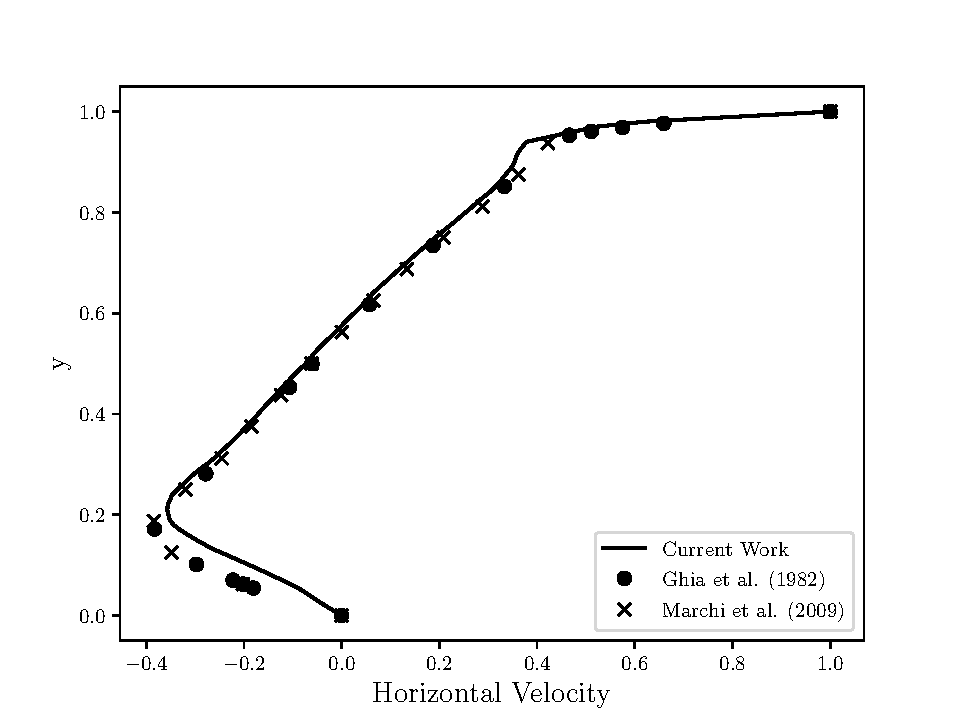
\includegraphics[scale=0.53]{./02_chaps/cap_validation/figure/Re_1000_u_profile.pdf}\\
      (d)
     \end{minipage}
     \medskip
     \caption{The tangential velocity $u$ profile in central line of cavity ($x=0.5$) for several Reynolds number:
     (a) 10
     (b) 100
     (c) 400
     (d) 1000.}
     \label{velocity vx cavity}
\end{figure}
\end{center}

\begin{figure}[H]
     \centering
     \begin{minipage}{.5\linewidth}
      \centering
      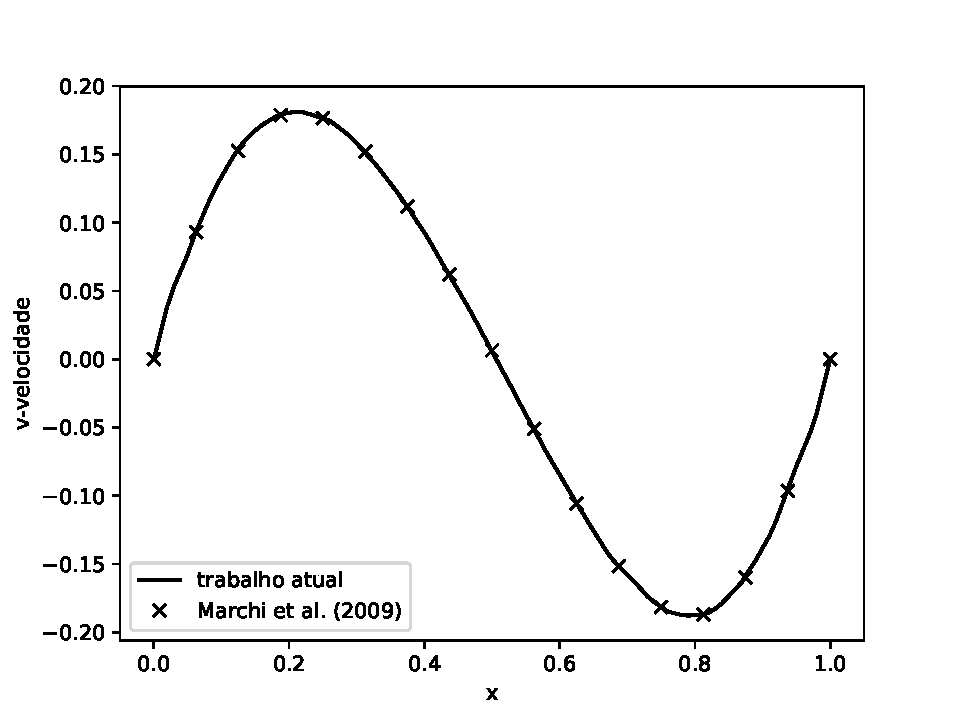
\includegraphics[scale=0.53]{./02_chaps/cap_validation/figure/Re_10_v_profile.pdf}\\
      (a)
     \end{minipage}%
     \begin{minipage}{.5\linewidth}
      \centering
      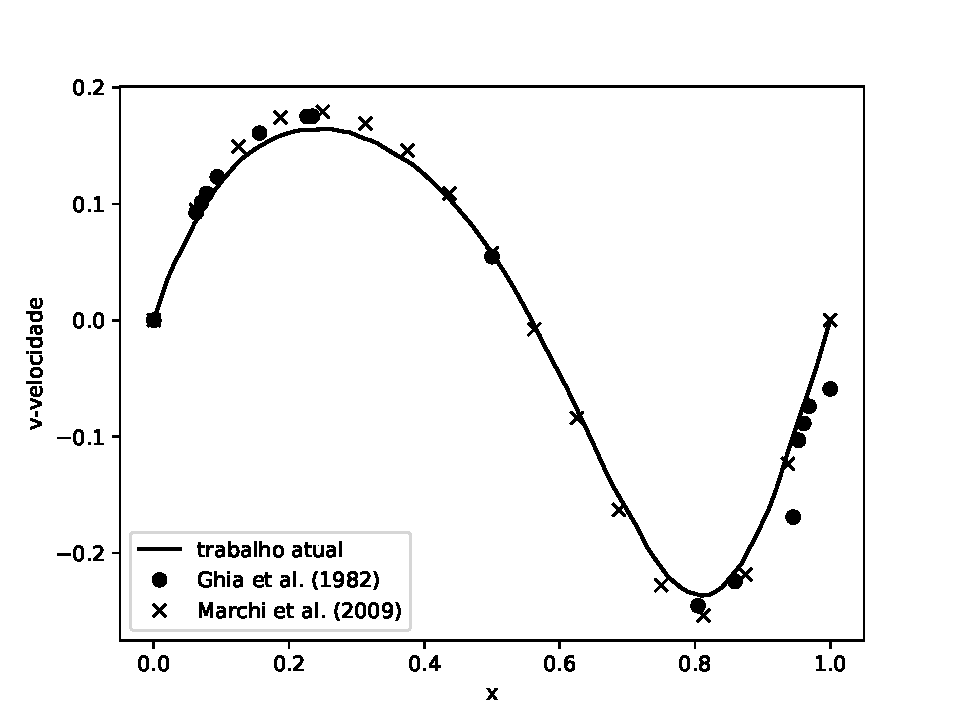
\includegraphics[scale=0.53]{./02_chaps/cap_validation/figure/Re_100_v_profile.pdf}\\
      (b)
     \end{minipage}
     \begin{minipage}{.5\linewidth}
      \centering
      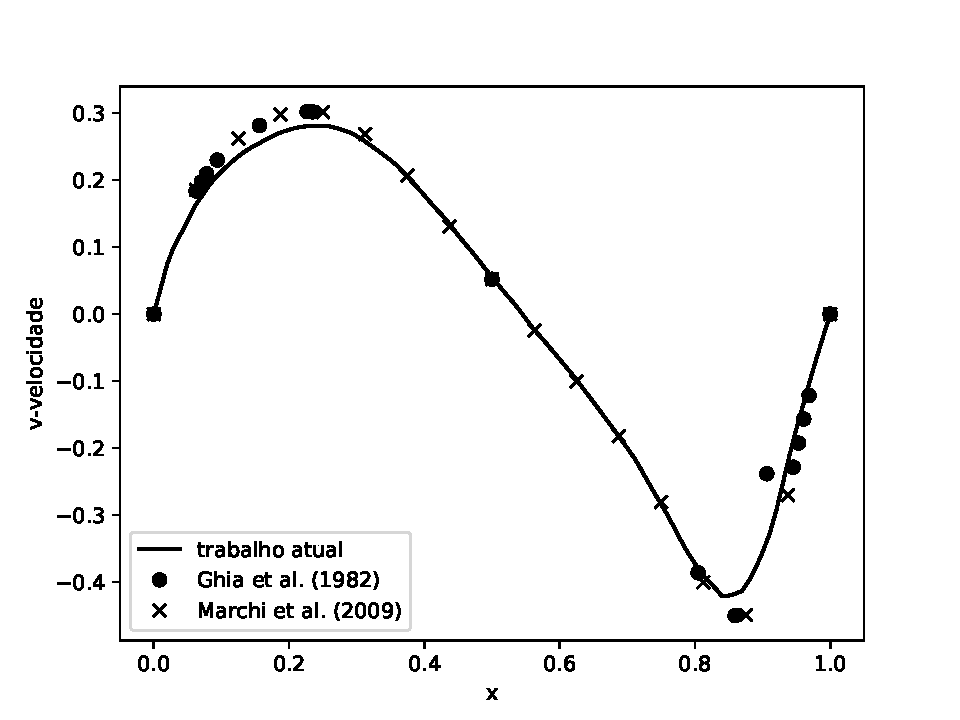
\includegraphics[scale=0.53]{./02_chaps/cap_validation/figure/Re_400_v_profile.pdf}\\
      (c)
     \end{minipage}%
     \begin{minipage}{.5\linewidth}
      \centering
      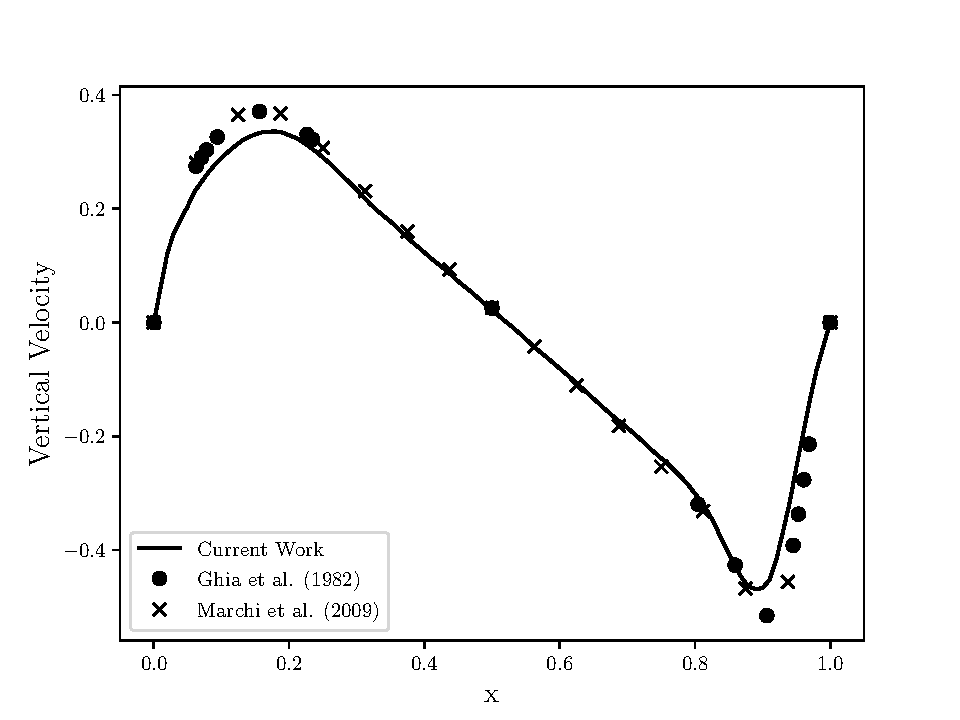
\includegraphics[scale=0.53]{./02_chaps/cap_validation/figure/Re_1000_v_profile.pdf}\\
      (d)
     \end{minipage}
     \medskip
     \caption{The normal velocity $v$ profile in central line of cavity ($y=0.5$) for several Reynolds number:
     (a) 10
     (b) 100
     (c) 400
     (d) 1000.}
     \label{velocity vy cavity}
\end{figure}

